%; whizzy chapter
% -initex iniptex -latex platex -format platex -bibtex jbibtex -fmt fmt
% 以上 whizzytex を使用する場合の設定。

%     Kansai Debian Meeting resources
%     Copyright (C) 2007 Takaya Yamashita
%     Thank you for Tokyo Debian Meeting resources

%     This program is free software; you can redistribute it and/or modify
%     it under the terms of the GNU General Public License as published by
%     the Free Software Foundation; either version 2 of the License, or
%     (at your option) any later version.

%     This program is distributed in the hope that it will be useful,
%     but WITHOUT ANY WARRANTY; without even the implied warranty of
%     MERCHANTABILITY or FITNESS FOR A PARTICULAR PURPOSE.  See the
%     GNU General Public License for more details.

%     You should have received a copy of the GNU General Public License
%     along with this program; if not, write to the Free Software
%     Foundation, Inc., 51 Franklin St, Fifth Floor, Boston, MA  02110-1301 USA

%  preview (shell-command (concat "evince " (replace-regexp-in-string "tex$" "pdf"(buffer-file-name)) "&"))
% 画像ファイルを処理するためにはebbを利用してboundingboxを作成。
%(shell-command "cd image200708; ebb *.png")

%%ここからヘッダ開始。

\documentclass[mingoth,a4paper]{jsarticle}
\usepackage{kansaimonthlyreport}
\usepackage[dvips]{xy}

% 日付を定義する、毎月変わります。
\newcommand{\debmtgyear}{2009}
\newcommand{\debmtgdate}{27}
\newcommand{\debmtgmonth}{12}
\newcommand{\debmtgnumber}{30}

\begin{document}

\begin{titlepage}

% 毎月変更する部分、本文の末尾も修正することをわすれずに

 第\debmtgnumber{}回 関西 Debian 勉強会資料

\vspace{2cm}

\begin{center}
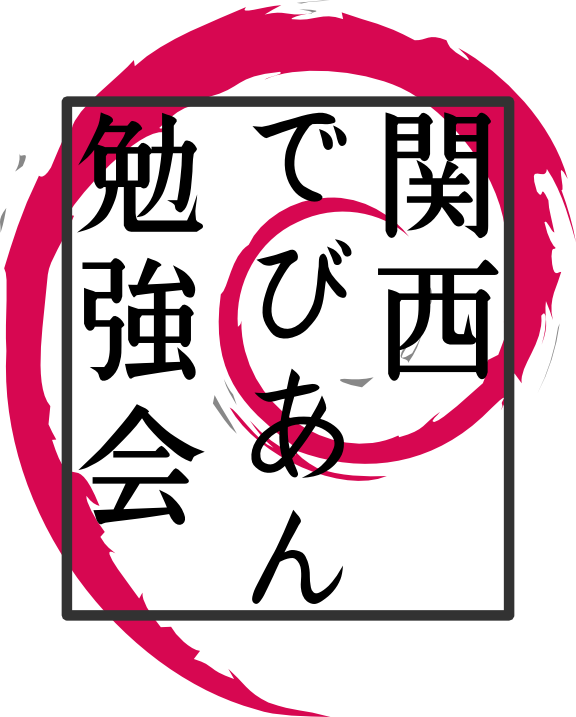
\includegraphics{image200802/kansaidebianlogo.png}
\end{center}

\begin{flushright}
\hfill{}関西 Debian 勉強会担当者 佐々木・倉敷・のがた \\
\hfill{}\debmtgyear{}年\debmtgmonth{}月\debmtgdate{}日
\end{flushright}

\thispagestyle{empty}
\end{titlepage}

\dancersection{Introduction}{Debian JP}
 
 関西 Debian 勉強会はDebian GNU/Linux のさまざ
 まなトピック(新しいパッケージ、Debian 特有の機能の仕組、Debian 界隈で起
 こった出来事、などなど)について話し合う会です。

 目的として次の三つを考えています。
 \begin{itemize}
  \item MLや掲示板ではなく、直接顔を合わせる事での情報交換の促進
  \item 定期的に集まれる場所
  \item 資料の作成
 \end{itemize}

 それでは、楽しい一時をお楽しみ下さい。

\newpage

\begin{minipage}[b]{0.2\hsize}
 {\rotatebox{90}{\fontsize{80}{80}
{\gt 関西デビアン勉強会}}}
\end{minipage}
\begin{minipage}[b]{0.8\hsize}
\hrule
\vspace{2mm}
\hrule
\setcounter{tocdepth}{1}
\tableofcontents
\vspace{2mm}
\hrule
\end{minipage}

\dancersection{最近のDebian関係のイベント報告}{Debian JP}

\subsection{オープンフォース Debian(非公式) 勉強会 徳島 200912 / のがたじゅ
ん}

\begin{wrapfigure}{l}{16zw}
 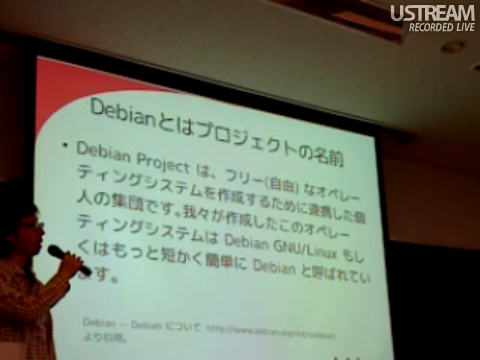
\includegraphics[width=16zw]{image200912/tokushima1.png}
\end{wrapfigure}

12月19日に徳島県の四国大学交流プラザで開催された、オープンフォース
Debian(非公式)勉強会 徳島 200912にお呼ばれしていってきました。

当日は寒波襲来、他のIT系勉強会とのバッティング、その他季節のイベントなど
があって、人が集まってくれるのだろうかと思いながら行ったのですが、10人以
上の人が集まってかなり盛り上がりました。

のがたは、「Debianと関西Debian勉強会の紹介」「あなたの知らないDebian
Live(改)」という二つの発表をしてきました。

「Debianと関西Debian勉強会の紹介」は、Debianユーザー向けに、Debianがユニ
バーサルなオペレーティングシステムを作るゆるやかな個人の集団であること、
Debian社会契約とDebianフリーソフトウェアガイドライン(DFSG)、Debianと
Debian JP、関西Debian勉強会について、バグ報告や翻訳からお手軽にDebianに参
加できるというお話をしました。

参加された人の多くは、すでにDebianを使っている方が多く、とても興味深く聞
いていただけたように思いました。

もう一つの発表「あなたの知らないDebian Live(改)」は、以前岡山で発表した
Debian Liveの周辺についての発表を、live-helper 2.0など最近の動きに合わせ
て変更した改訂版を発表しました。

改訂版の発表だけでは申し訳ないので、デモとしてDebian Liveが起動するとフル
スクリーンでqemuが起動し実機を動かしているように仮想マシンが使える
qlive\footnote{\url{http://github.com/nogajun/qlive}}で、Windows98が使え
るデモをしました。

こちらはデモ直前にクラッシュするという出来事がありましたが、なんとか復旧
させてお見せすることができウケたので、よかったなと思いました

徳島は夏と今回の冬に行って、徳島大学や四国大学の学生のDebianユーザーが多
いことが改めて実感できたので、また機会を見て訪れようかと思います。


\dancersection{ハンドメイドGPSロガーの構築}{まさ}

\subsection{はじめに}

これまでDebianのインストール、環境整備、ウェブアプリケーションのシステム
構築をするなどシステムを触ることはある程度経験したものの、お小遣い帳サー
バや、GPSロガーなど、何らかの実用になるものはなかなかつくれませんでした。

そこでプログラムのスキルを得るための教材として、GPSロガーを作成したので、
報告します。

これからDebianを目指す人の興味を惹き、手がかりとなって少しでもお役に立て
れば幸いです。

\subsection{GPSとは}
”Global Positioning System”は数十個の衛星からの電波を受信して現在位置を割り出すシステムです。

原理等はいろんな書籍やインターネットに掲載されているようですので、ここでは説明を割愛します。

\subsection{GPSロガーのハード構成}
必要なハード構成は以下の通りです。

今回実際に使用したハードの概略仕様はAppendixを参照してください。
\begin{center}
        \framebox[6.5zw]{ネットブック}
        \hspace{1em}$\Longleftarrow$\hspace{1em}
        \framebox[7.5zw]{PS2-USB変換}
        \hspace{1em}$\Longleftarrow$\hspace{1em}
        \framebox[7.5zw]{GPSレシーバ}        
\end{center}

\begin{enumerate}
 \item GPSレシーバ \\
            GPSアンテナ、受信回路、信号送出回路から成り、 PS2コネクタからシリアルにキャラクタ文字でGPS情報が送出されます。
 \item PS2-USB変換 \\
            GPSレシーバから信号送出用のシリアルインタフェースをUSBインタフェースに変換するためのものです。変換ケーブルになっています。
 \item ネットブック \\
            USBインタフェースで受信したGPS情報を受け取り、ファイルに溜め込みます。また、GPS情報をいろいろ加工して楽しめます。
\end{enumerate}

\subsection{ネットブックセットアップ概要}
ネットブック購入直後からGPSロガーを構築する場合について概要を説明します。

\begin{enumerate}
      \item Debian Base systemのインストール \\
    Debian-netinst-isoを使ってBase systemをインストールします。
      \item X Window Systemのインストール
      \item Gnomeのインストール
      \item 日本語入力システムのインストール \\
    プログラム作成時必要です。今回は、”uim-anthy”をインストールしました。
      \item NTPのインストール \\
    システム時刻自動調整用のプログラムです。
    今回はGPSを扱うため、特にシステム時刻が大切になると思われます。
      \item プログラム言語のインストール \\
    GPSロガーアプリケーション作成に必要です。
    今回は、とっつきやすく、GUIができ、
    ライブラリが豊富と言われる”Python”(バイトンor パイソン?)
    を選択しました。
    私にとって、確かにとっつきやすいですが、それなりに苦労しました。
    pythonのせいではなく、プログラミングというもの自体、
    思ったものがそう簡単にできるわけではないということだと思われます。
      \item Python libraryのインストール
    \begin{enumerate}
          \item PySerial \\
        シリアルポート入出力用のプログラムです。
          \item Python Tkinter \\
        GUIプログラミング用のひとつです。
          \item datetime \\
        時刻を扱うとき使います。
          \item os, os.path \\
        ファイルの開閉、読み書きするとき使います。
          \item sys(場合によって使用) \\
        コマンドパラメータを取得するとき使います。
    \end{enumerate}
\end{enumerate}

\subsection{GPSデータ出力形式}
今回使用したGPSレシーバはNMEA0183というプロトコルです。
NMEA0183では以下のような形式などでデータが出力されますが、

\begin{description}
 \item[GLL] Geographic Position, Latitude and Longitude
 \item[GSA] GNSS DOP and Active Satellites
 \item[RMC] Recommended Minimum Specific GNSS Data
\end{description}

今回は

\begin{description}
 \item[GGA] Global Positioning System Fix Data
\end{description}

という形式のみ利用しました。
\clearpage
GGA形式の仕様は次の通りです。

\begin{commandline}
GGA,123519.00,4807.038247,N,01131.324523,E,1,08,0.9,545.42,M,46.93,M,5.0,1012*42
123519.00 	= 測位時刻(UTC) 12:35:19.00
4807.038247,N 	= 緯度 48度07.038247分(北緯)
01131.324523,E 	= 経度 11度31.324523分(東経)
1 	= GPSのクオリティ; 0 = 受信不能、1 = 単独測位、2 = DGPS
08 	= 受信衛星数
0.9 	= HDOP
545.42, M 	= 平均海水面からのアンテナ高度(m)
46.93, M 	= WGS-84楕円体から平均海水面の高度差(m)
5.0 	= DGPSデータのエイジ(秒)
1012 	= DGPS基準局のID
*42 	= チェックサム
\end{commandline}

ここから、時刻、緯度、経度などのデータを利用しました。

\subsection{アプリケーション作成}
いよいよアプリケーションの作成です。
上のGPS GGAデータを加工して、表示したり、ログをとります。


\subsection{実行}
アプリケーションを走らせます。

\subsection{今後の抱負}
今回のアプリケーションを基にいろんな展開が考えられます。
Sunday programmerとして今後も少しづつであっても、根気よく前進します。
\begin{enumerate}
      \item Open Street Mapへの貢献 
      \item Open Street Mapの利用
\end{enumerate}
地図上への現在位置の表示や、ログデータからトレース表示したりと地図情報は重要です。
この場合、種々の縮尺の地図が必要ですが、Open Street Mapはベクトルデータであることからこの点が有利です。
また、ナビのように指定した位置の地図を得る場合、これが可能なインタフェースがOSMにあれば(あるのかも知れませんが)、より柔軟に利用できるのではないかと期待しています。

\subsection*{Appendix}
% \subsubsection*{仕様}
[A] ネットブック仕様概略
\begin{commandline}
PC:       Asus EeePC 901 
CPU:      Intel Atom (1.6GHz) 
Memory:   1GB 
HDD(SSD): 4GB + 8GB 
Monitor:  8.9型、1024 x 600 
I/F:      USB 2.0 
\end{commandline}
[B] ネットブックシステム仕様 
\begin{commandline}
OS:      Debian Lenny 
Kernel:  2.6.26-2-686 
言語:    Python 2.5.2 
Library: pySerial, tkinter等 
\end{commandline}
\clearpage
[C] GPSレシーバ仕様 
\begin{commandline}
型式:       GPS-S103(Wonde proud社製)
位置 精度:  5 - 25m CEP without SA
時刻精度:   1μs synchronized to GPS time 
プロトコル: NMEA0183
動作温度:   -40 °C ~ +85 °C 
動作湿度:   5% to 90% (結露なき事) 
電源:       DC 3.7 ~ 6V, typical 5V(今回はUSBより供給)
I/F:        TTL serial(PS2コネクタ). USB option 
\end{commandline}
[D] GPSロガー実行例
\begin{enumerate}
\item ログファイル
\begin{commandline}
$GPVTG,113.96,T,,,0.00,N,0.00,K,A*7C 
$GPGGA,054832.084,3450.2455,N,13615.2118,E,1,09,01.0,253.6,M,37.3,M,,*6B 
$GPRMC,054832.084,A,3450.2455,N,13615.2118,E,0.00,113.96,260909,,,A*6C 
$GPVTG,113.96,T,,,0.00,N,0.00,K,A*7C 
$GPGGA,054833.083,3450.2455,N,13615.2118,E,1,08,01.1,253.5,M,37.3,M,,*6E 
$GPRMC,054833.083,A,3450.2455,N,13615.2118,E,0.00,113.96,260909,,,A*6A 
$GPVTG,113.96,T,,,0.00,N,0.00,K,A*7C 
$GPGGA,054834.083,3450.2455,N,13615.2118,E,1,09,01.0,253.4,M,37.3,M,,*68 
$GPGSA,A,3,03,06,07,08,11,16,19,22,25,,,,2.2,1.0,1.9*39 
$GPGSV,3,1,09,3,44,055,37,6,33,060,33,7,50,266,39,8,28,311,37*7A
\end{commandline}
\item 現在位置データ表示例
\begin{figure*}[h!]
    \centering
    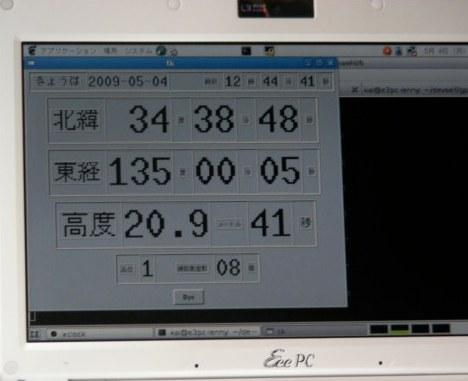
\includegraphics[scale=0.6]{image200912/handmadegpsloger1.jpg}
\end{figure*}
\item 現在位置地図表示例
\begin{figure*}[h!]
    \centering
    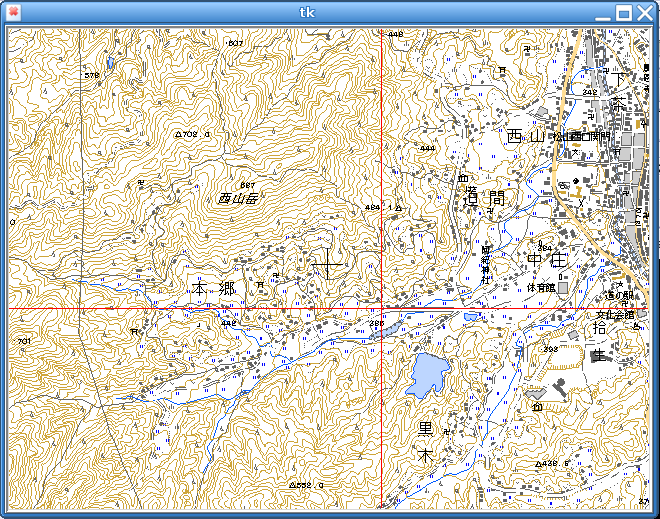
\includegraphics[scale=0.6]{image200912/handmadegpsloger2.png}
\end{figure*}
\clearpage
\item プログラム例 (抜粋)
% \subsubsection*{プログラム例}
% (抜粋ですのでこのままでは動作しません)
\begin{commandline}
#!	/usr/bin/python2.5 
# -*- coding: utf8 -*- 

#******************************************** 
#	 
#	コード例 for KDM 2009.12.27	 
#	 
#	Now edited on .... 2009-02-07 ... 
#	Reviced on    .... 2009-12-23 
#	 
#******************************************** 

# 必要なモジュールをインポート
import os.path 
import Tkinter as Tk 
import time, datetime 
import	serial 
import	string 
	. 
	. 
	. 
# GUI バッファ準備
root = Tk.Tk() 
buff_date = Tk.StringVar() 
buff_date.set(honjitsu) 

buff_hT = Tk.StringVar() 
buff_mT = Tk.StringVar() 
buff_sT = Tk.StringVar() 
buff_hT.set('') 
buff_mT.set('') 
buff_sT.set('') 
	. 
	. 
	. 
# 表示欄の作成
# display date &  gpstime 
f0 = Tk.Frame(master=None, relief= 'ridge', bd=3) 
bd0 = Tk.Label(f0, text="きょうは", font=dfont12, relief = 'ridge') 
bd1 = Tk.Label(f0, textvariable = buff_date, font=dfont18, relief = 'ridge') 
bd2 = Tk.Label(f0, text="    ", font=dfont12, relief = 'flat') 
b00 = Tk.Label(f0, text="時刻", relief = 'ridge') 
b01 = Tk.Label(f0, textvariable = buff_hT, font=dfont18, relief = 'ridge') 
b02 = Tk.Label(f0, text="時", relief = 'ridge') 
b03 = Tk.Label(f0, textvariable = buff_mT, font=dfont18, relief = 'ridge') 
b04 = Tk.Label(f0, text="分", relief = 'ridge') 
b05 = Tk.Label(f0, textvariable = buff_sT, font=dfont18, relief = 'ridge') 
b06 = Tk.Label(f0, text="秒", relief = 'ridge') 

for e in [ bd0, bd1, bd2, b00, b01, b02, b03, b04, b05, b06 ]: 
	e.pack(side='left', padx=5) 

# display latitude 
f1 = Tk.Frame(master=None, relief= 'ridge', bd=3) 
b10 = Tk.Label(f1, text="北緯", font=dfont24, relief = 'ridge') 
b11 = Tk.Label(f1, textvariable = buff_dLa, font=dfont48, relief = 'ridge') 
b12 = Tk.Label(f1, text="度", relief = 'ridge') 
b13 = Tk.Label(f1, textvariable = buff_mLa, font=dfont48, relief = 'ridge') 
b14 = Tk.Label(f1, text="分", relief = 'ridge') 
b15 = Tk.Label(f1, textvariable = buff_sLa, font=dfont48, relief = 'ridge') 
b16 = Tk.Label(f1, text="秒", relief = 'ridge') 

for e in [b10, b11, b12, b13, b14, b15, b16 ]: 
	e.pack(side='left', padx=5) 
	. 
	. 
	. 
# 1秒毎の表示定義関数
def showtime(): 
	# open log file for write gps data 
	f = open( fname, 'a') 
	gpstime = '' 
	# get 'GPGGA' sentence from gps receiver. 
	# USBシリアルラインのオープン
	ser = serial.Serial('/dev/ttyUSB0', 4800, timeout = 3) 
	print ser.portstr 
	line = ser.readline() 	# 1行づつ読み込み
	words = line.split(',') 
	while( not words[0] == '$GPGGA'): 
		line = ser.readline() 
		words = line.split(',') 
	print line 
	ser.close() 

\end{commandline}
\clearpage
プログラム例, 続き
\begin{commandline}
	# time # 時刻データの切り出しと変換
	time = words[1] 
	hT_utc = time[:2] 
	hT_jst = str( ( int(hT_utc) + 9 ) % 24 ).zfill(2) 
	mT = time[2:4] 
	sT = str( int( float(time[4:]) ) ).zfill(2) 
	gpstime = 'gpstime  = ' + hT_jst + ':' + mT + ':' + sT + ' JST' 
	. 
	. 
	. 
	# latitude # 緯度データの切り出しと変換
	lati = words[2] 
	deg_lati = " " + lati[:2] 
	min_lati = lati[2:4] 
	sec_lati = str( int(float(lati[4:]) * 60 ) ).zfill(2) 
	gpslati = 'latitude = ' + deg_lati + ':' + min_lati + ':' + sec_lati + ' ' + words[3] + '  ' 
	# longitude # 経度データの切り出しと変換
	long = words[4] 
	deg_long = long[:3] 
	min_long = long[3:5] 
	sec_long = str( int(float(long[5:]) * 60 ) ).zfill(2) 
	gpslong  = 'longitude=' + deg_long + ':' + min_long + ':' + sec_long + ' ' + words[5] + '  ' 
	# koudo 
	kodo = words[9] 
	gpskodo  = 'koudo= ' + kodo + ' m' 
	. 
	. 
	. 
	# write new data to data file 
	f.write(line) 		# ログデータのファイルへの書き込み

	f.close 

	root.after(1, showtime) # 1秒毎に表示を更新

showtime() # 表示関数の起動
root.mainloop() # 無限ループ
\end{commandline}
\end{enumerate}

\clearpage
\dancersection{Debian を使って愉しむ Open Street Map 入門}{たなかとしひさ}

\subsection{Open Street Map をご存知ですか?}

\begin{figure*}[h!]
    \centering
    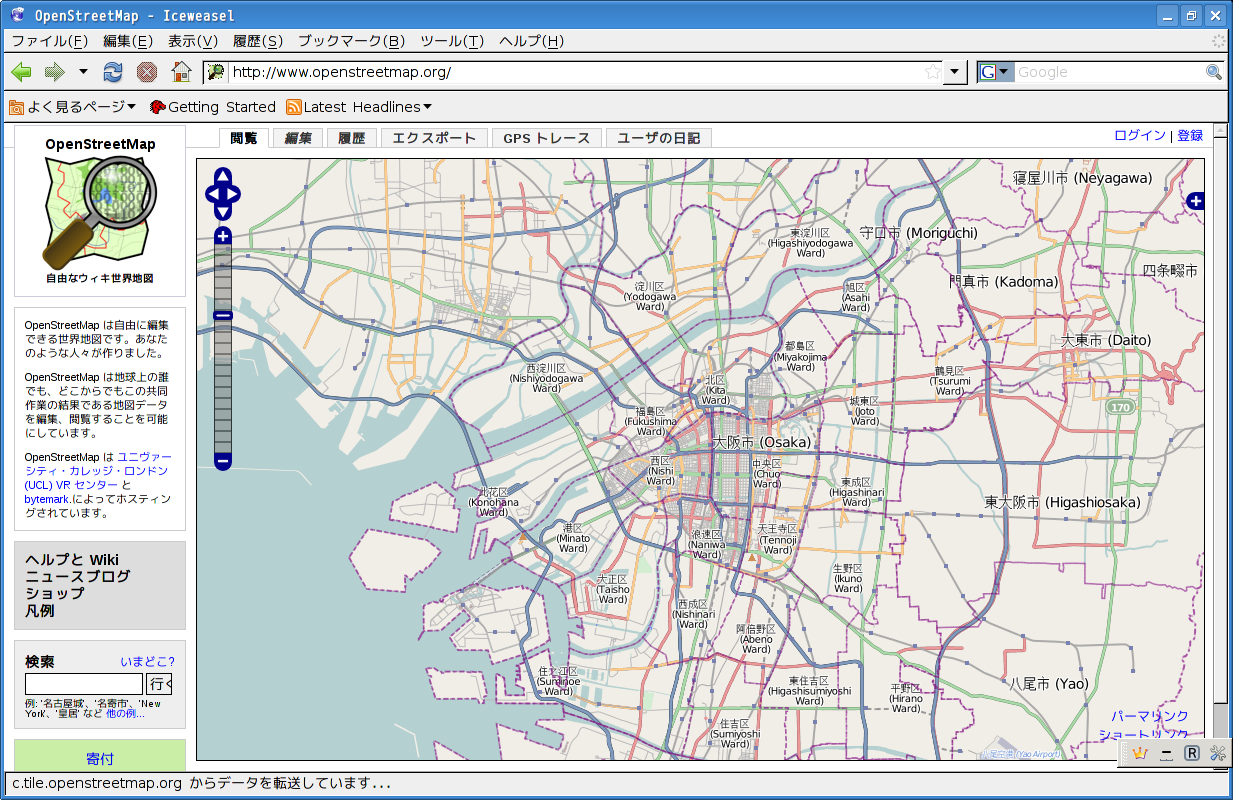
\includegraphics[scale=0.3]{image200912/debianosm1.png}
\end{figure*}

2009年度12月のDebian 勉強会のお知らせで、
\url{http://www.openstreetmap.org/} にアクセスして、お住まい近辺の地図を
見て頂けたらと案内しました。

ご覧になられた皆さん、感想はいかがでしょうか。

「すげぇ、素晴らしい!」

「Google Map の廉価版?」

「Debian と何の関係があるのさ?」

 等など、色々な感想があると思います。

今回の勉強会では、Debian System の応用として、Debian を使って、この
OpenStreetMap(以降、OSM と表記)について、一緒に勉強していきましょう。

\subsection{免責}
\begin{itemize}
 \item このテキストは、たなかとしひさ(tosihisa@netfort.gr.jp)が書いたものです。
 \item このテキストには、間違いがあるかもしれません。
 \item 記載内容は、できるだけ最新(2009年12月)の事情にあわせて記載したつもりですが、時間の経過で内容が変化する場合があります。
\end{itemize}

\subsection{OpenStreetMap(OSM) って何ですか?}
\url{http://wiki.openstreetmap.org/wiki/Ja:Main_Page} からの引用です。

\begin{quotation}
OpenStreetMapは道路地図などの地理情報データを誰でも利用できるよう、フリー
の地理情報データを作成することを目的としたプロジェクトです。自由に使える
と思っている地図の多くが実は法的・技術的に問題があり、人々がクリエイティ
ブに、生産的に、あるいは今まで予期しなかった方法でそれを 利用する事を妨げ
ているため、このプロジェクトは開始されました。
\end{quotation}

\subsection{Debian System と OSM}

今回の関西 Debian 勉強会は、従来のテーマとは異なり、異色でもあります。
「OSM って、Debian と何か関係あるの?」と言われると、確かに強い関係…
はありません。

しかし、Debian System と OSM を組み合わせる事で、

\begin{center}
 \textbf{{\large「自由度の高い」地図ソフト環境} }
\end{center}

が実現できます。これは、画期的な事だと筆者は考えています。

Debian Systemで、どれだけ素晴らしい地図ソフトが .deb になって apt で得ら
れるとしても、地図データが無ければ魅力を欠きます。

Debian System を始めたとした Linux ディストリビューションは、「自由に使う
事が出来るコンピュータソフトウェア環境」を実現できるものですが、それと
OSM とを組み合わせる事で、自由に使う事が出来るコンピュータソフトウェア環
境の中に、「地図の閲覧」を含める事が出来ます。

Debian System もそうであるように、OSM もまた、「一部の特権階級」のもので
はありません。望めば、誰でもが自由に使う事が出来ます。
OSM は、使うには一苦労かかる事もしばしばありますし、地図自身、日本国内で
は十分に揃っているとは言えない状況です。

しかし、誰でもが、自由に使える地図データを提供できる事は、Debian が目指す
ゴールと重なります。

また、「単に Debian を使う」だけでなく、Debian の応用事例を増やす事は、
Debian コミュニティに取っても有益と考えています。
Debian System は、サーバ、医療、組込みなど、様々な分野で使われています。
その中に「自由に使える地図環境」を加える事が出来ます。

\subsection{OSM のライセンス}

OSM の地図データは、Creative Commons Attribution-ShareAlike 2.0、簡略系
で書くと CC BY-SA (表示-継承)です。
\footnote{\url{http://wiki.openstreetmap.org/wiki/Ja:OpenStreetMap_License}}

なお、OSM の地図データのライセンスは、2009年12月現在 Open Database License (ODbL) への移行が検討されています。
\footnote{\url{http://wiki.openstreetmap.org/wiki/Ja:Open_Database_License}}

12月の関西 Debian 勉強会実施頃には、もしかするとライセンスが変更されているかも知れません。

\textbf{{\large *急募*} }

日本の OSM コミュニティは、ODbL に関する情報を必要としています。
ODbL に詳しい(出来れば)日本語の情報がありましたら、筆者までお知らせ下さいますと助かります。

ODbL は、日本ではまだ認知が低いためか、日本語の情報が少なく、どの様な情報
でも構いませんので、筆者までお知らせ下さいますと助かります。

\subsection{OSM の特徴}

\subsubsection{OSM の地図データは、ビットマップではなくベクトルデータ}

OSM の地図データはベクトルデータです。
\url{http://www.openstreetmap.org/} や、\url{http://osm.jp/} から参照でき
る地図画像は、そのベクトルデータをビットマップデータへレンダリングしたも
のです。

地図データがベクトルデータなので、地図の表現能力自身は、ビットマップに比
べると劣りますが、ベクトルデータの場合、拡大・縮小が自由に行える事と、ルー
ト探索が可能になります。

OpenStreetMap の地図データを用いたルート探索サービスを提供しているサイト
の一つに、CloudMade があります。
CloudMade の地図サイト (\url{http://maps.cloudmade.com/}) にアクセスして、
大阪(梅田)から、関西 Debian 勉強会までのルート探索結果を下記に示します。

\begin{figure}[h]
 \centering
 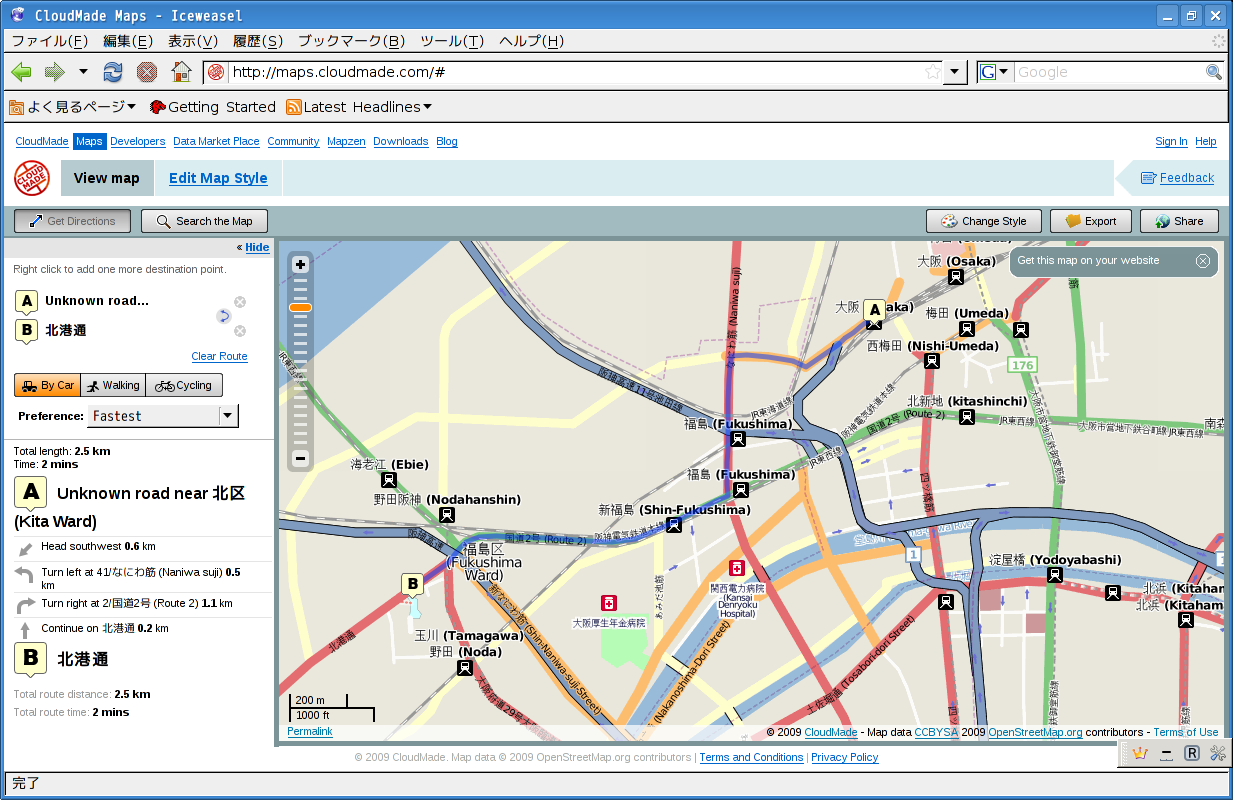
\includegraphics[scale=0.4]{image200912/debianosm2.png}
 \caption{CloudMade による関西 Debian 勉強会へのルート探索図}
\end{figure}

OSM の地図データ自身がまだまだ不足している事と、地図データの精度が足りな
いので、期待したルート探索結果にはまだならないかも知れませんが、この様な
ルート探索が行える可能性を OpenStreetMap は持っています。

\subsubsection{地図データの作成は、アカウント登録さえすれば誰にでも可能}

\begin{wrapfigure}{r}{30zw}
 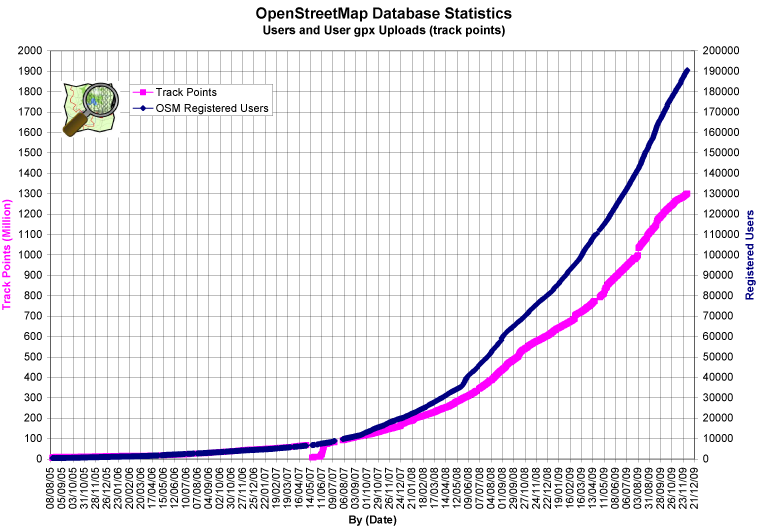
\includegraphics[scale=0.5]{image200912/debianosm3.png}
 \caption{OSM登録者数と作図データの推移グラフ}
\end{wrapfigure}

OSM の地図データの作成は、OSM へのアカウントを登録すれば誰にでも作成、編
集が可能です。

2009年5月に、OSM ユーザ数は 100,000 を越えました。右に、その登録者数と
作図データの推移グラフを示します。
(出典:\url{http://www.opengeodata.org/2009/03/17/osm-passes-100000-users/})

\clearpage

\subsubsection{Wiki の考え方をベースにしている}

地図データの作成は、Wiki の考え方が根本にあります。A さんが作図したデータ
を B さんが修正する事が可能です。
Wiki の悪い面 いわゆる「荒らし」的な事も、やろうと思えば出来てしまいます
し、地域によっては「編集合戦」があるのも事実です。

しかしながら、Wiki ベースであるので、「より良い方向に向かって修正する」事
が可能であり、例えば一方通行の方向が逆である事を見つけた場合、アカウント
を持っていれば修正する事が出来ます。

\subsubsection{地図データはオフラインでも利用できる}

GoogleMap は実に便利ですが、基本はオンライン、要するにインターネットに繋
がっている環境下である事が前提にあります。
また、GoogleMap が提供する地図は、事前に Google の書面に同意を得る事無し
に独自の技術によるアクセスや地図の複製は出来ません。

出典:
\begin{itemize}
 \item \url{http://www.google.co.jp/intl/ja_jp/help/terms_maps.html}
 \item \url{http://www.google.com/intl/ja_ALL/help/terms_local.html}
\end{itemize}

これは、オフライン対応地図閲覧ソフトは、Google Map の地図データを書面によ
る同意無しに使えない事を意味します。
オフラインでも地図を閲覧できるソフトに Mobile GMaps
(\url{http://www.mgmaps.com/}) があります。これはオンラインでもオフラインでも使
用できる PDA や SmartPhone 向け地図ソフトですが、上記の理由から、このソフ
トは Google Map の地図に対応していません。

誤解の無い様に付け加えると、筆者は GoogleMap のあり方は問題視していません。
GoogleMap が提供するサービスは、これらを補うに十分と考えています。

大事な事は、インターネットがどこでも安価に使える様になったとは言え、それ
は「全世界から見ればごく一部」でしか無いと言う事です。
日本でも、山間の地域に行くと、携帯も圏外になる場合があります。

この様な場合でも、地図データをオフラインで持っておけば、圏外でも地図を閲
覧できますし、圏内でもパケット課金を気にする必要はありません。

OSM の地図データをオフラインで見られるソフトの一つに、navit
(\url{http://wiki.navit-project.org/index.php/OpenStreetMaps}) があります。
navit は後の章で紹介します。

\subsection{(今だけの愉しみですが)走行ログになります}

筆者はバイクに乗り、アチコチに移動するのが趣味で、GPS を持って出かけてロ
グを取って後で眺めたりします。その時、「単にログを見る」だけではなく、
「そのログを元に地図を作図する」事が出来れば、さらにより良いと考えていま
す。

筆者が OSM に地図データをコミットし始めた頃は、大阪は殆ど何もありませんで
した。記憶ですが、名神か阪神高速の一部があった程度です。どなたか、大阪を
通過された方が作図されたのだと思います。

筆者はまず、大阪のシンボル御堂筋を作図しました。続けて、四ツ橋筋を作図し
ました。当時は「広大な白地図」でしたので、どこを走っても作図できましたが、
最近の大阪の OSM 地図の発展は目覚しく、少し考えてログを取らないと、誰かが
既に作図済みの所を走っているだけになります。

近畿地方で最も OSM の作図が進んでいるのは、滋賀県長浜市の OSM 地図と考え
ています。
滋賀県長浜市の OSM 地図発展は目覚しいもので、「よくぞここまで作図したもの
だなぁ・・・」と感嘆する事しきりです。

筆者は、「自由に使える地図を【使いたい】」と言う理由で OSM に注目し始めま
した。が、ミイラ取りがミイラと言う訳ではありませんが、目的が「自由に使え
る地図を【作ること】」に変ってきているのも事実です。

\subsection{OSM へのコミットは、地域社会への貢献にもなりえます。}

筆者は常々、事 OpenSource の成果は、地元社会にもつながればと考えています。

プログラミング言語 Ruby は、島根県の IT ならびに OpenSource 促進に良い影
響を与えたと考えています。OSM は、それと同じ効果を持ちえると考えています。

「地図」と言うのは、OpenSource コミュニティに限らず、誰にでも一応の興味が
あります。私の母はコンピュータ環境と無縁な生活を送りつづけていますが、母
は山歩きが趣味なので地図帳は持っています。

また、日本は地震が多いので、避難場所への地図を載せた看板を目にすると思い
ます。
筆者は、OSM が地震等の災害発生時に役に立つ日が来ればと考えています。
地震等の災害で、道路が分断された場合、どこからどこまでが通行不可なのかど
うかを、迅速に反映できる仕組みを、OSM は持っていると考えます。

また、視力が弱く、地図を見る事が出来ない場合にも、OSM の地図をベースに
「触地図」を作ってみたケースがあります。

現在の OSM の地図データは、日本国内で見れば、まだまだ足りないのが現状です
が、「地図」は殆どの人には、少なからず関係があるものですので、

この様に、様々な形での応用を OSM は持っています。

\subsection{OSMへの参加}

OSMへの参加は、
\url{http://wiki.openstreetmap.org/wiki/Ja:Beginners_Guide}を参考にすると
良いでしょう。基本的には下記の事をしていきます。

\subsubsection{OSMアカウントの作成(初めの1回だけ)}

\url{http://www.openstreetmap.org/create-account.html}にアクセスして、
OSMアカウントを作成します。同時に、
\url{http://wiki.openstreetmap.org/index.php?title=Special:UserLogin&type=signup&uselang=ja}
にアクセスして、OSM の Wiki アカウントを作成しておくと良いでしょう。

OSMは、地図データのアップロードは「OSMアカウント」を用いますが、それ以外
にも OSM の Wiki ページ(\url{http://wiki.openstreetmap.org/})がありますの
で、OSMに関する情報公開に用いると良いでしょう。

アカウントの作成は初めの1回だけですが、後々のGPSログのアップロードや作図ではOSMアカウント情報が必要です。

OSM作図の流れ図を下記に示します。

\begin{figure}[h]
 \centering
 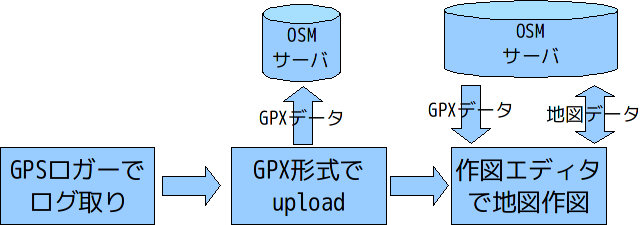
\includegraphics[scale=0.7]{image200912/debianosm4.png}
\end{figure}


\subsubsection{GPSロガーでログ取り}

GPSロガーを持って、まだ地図データの無い白地図の所に行き、GPS データをログ
していきます。

「マッピングパーティ」と言う催しがあります。これは、OSM同好の集まりでGPS
等を持ってログを取る催しです。この「マッピングパーティー」に参加するのも
良いでしょう。

\subsubsection{GPSログデータをアップロードする}

GPSロガーのデータをGPX形式にして、OSMサーバにアップロードします。

技術的には、GPSログデータをアップロードしなくても作図そのものは可能ですが、「GPSを元にした道である事」への根拠として、GPSログデータはアップロードしておいた方が良いでしょう。

\subsubsection{地図データを作成、編集する}

\begin{figure}[h]
 \centering
 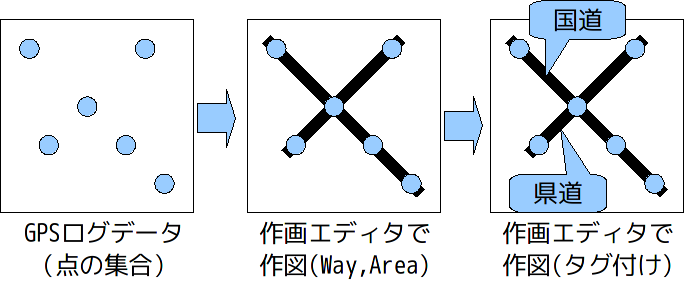
\includegraphics[scale=0.7]{image200912/debianosm5.png}
\end{figure}

GPSログデータを元に、OSM作画エディタを使って、実際に作図していきます。

GPSログデータは、点データの集合ですので、それをOSM作図エディタで繋いで行き、線にしていきます。

次に、その線データが国道なのか、県道なのか、一方通行かどうかの情報を付加していきます。これを、「タグ付け」と言います。
作図のイメージを下記に示します。

\subsubsection{マップを描画する! }
出来上がった地図を見てみましょう!
地図のレンダリングには少し時間がかかりますが、早ければ1時間位でレンダリングされます。

\subsection{OSM へ参加するには、GPSロガーは不可欠なの?}

GPSロガーが無いからと言って、OSMに参加できない事はありません。GPSロガーが無くても、下記の形でOSMへコミットできます。

\begin{itemize}
 \item 使ってみる。\\
OSMは地図データですので、実際にそれが現実とあっているかが重要です。とにもかくにも、OSMを使ってみて下さい。Debian System と同様に、「それを使う」だけでも、貢献として充分なのです。
 \item 間違いを修正する。\\
OSMの作図は、できるだけ正しくなるように作図が進んでいますが、例えば一方通行の方向が逆だったり、国道/県道の番号が間違っている場合もあります。
この様な場合、作画エディタでOSMデータをダウンロードできますので、間違いのある部分をダウンロードして修正してアップロードすれば、間違いが修正できます。
\end{itemize}

\subsection{Debian System 上で使える OSM (GIS) 関連ソフト}
 Debian Systemは、メンテナの尽力により豊富なバイナリパッケージを使う事ができますが、
 OSM 関連で利用できるソフトウェアを下記に示します。もちろん、これだけではありません。
 私見ですが、GPS を扱うソフトは、Windows よりも Debianの方が多岐に渡っていると感じています。

\subsubsection{gpsd}

\begin{commandline}
# apt-get install gpsd
\end{commandline}

gpsd は、OSMでは必須では無いのですが、Debian や Linux でGPSデータを受信する際にほぼ標準として使われているので紹介します。
このソフトは、GPS 受信機と PC を接続し、NMEA-0183 センテンスまたは GPS の独自プロトコルと通信し、現在の緯度経度、UTC 時間を処理します。

Debian System 上で動作する地図関連のソフトは、GPS 受信機と直接通信せず、gpsd を経由して緯度経度の情報を得るものが多いです。
gpsd を経由させる事で、GPS 受信機一つに対し、複数の(GPS を必要とする)ソフトが使えるようになります。

\begin{figure}[h]
 \centering
 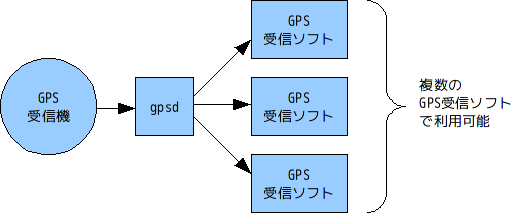
\includegraphics[scale=0.9]{image200912/debianosm6.png}
\end{figure}

また、gpsd は、NTP サーバ向けの時刻源としても機能します。NTP(ntpd) とは、共有メモリドライバを介して行います。ただし、gpsd を NTP サーバ向けの時刻源にしても、NTP 階層の Stratum 1 の精度になるわけではありません。これは、gpsd が時刻情報を受信する時、共有メモリに書き込むときに「ゆらぎ」が生じるからです。

Debian System と OSM からは少し外れますが、もし、GPS を時刻源として Stratum 1 相当の NTP サーバを作るならば、"1PPS (one pulse per second)" 出力つき GPS が必要になります。

1PPS とは、「正確に1秒のパルス」を発生するもので、このパルスを Linux カーネルで捕まえる事で、時刻のゆらぎを少なくします。

\subsubsection{gpsbabel}

\begin{commandline}
# apt-get install gpsbabel
\end{commandline}

gpsbabel は、様々な GPS データの形式を変換するソフトです。

GPS データの「基本的な仕様」としては、NMEA-0183 センテンスがその基本なの
ですが、GPS 受信機ベンダーは、独自フォーマットでデータを保存する場合があ
ります。それは様々なGPSベンダーから、様々なデータ形式があります。Google
Earth の “.kml”形式も、そのGPSログの保存形式の一つです。

gpsbabel は、その GPS データ形式を変換するソフトです。

OSMが採用しているGPSログ形式は、<time>タグ付きGPX形式のみですので、もし
GPS受信機、あるいは付属ソフトが<time>タグ付きGPX形式に対応していない場合、
gpsbabelで変換しなければならない場合があります。

参考に、NMEA-0183 センテンスのGPSログデータを GPX に変換するには、下記の
様に実行します。

\begin{commandline}
$ gpsbabel -w -r -t -i nmea -f {nmea-log-file} -o gpx -F {GPX_DATA}.gpx
\end{commandline}

\clearpage

\subsubsection{Merkaartor (発音は"メルカトル"です)}

「deb \url{http://www.backports.org/debian} lenny-backports main contrib non-free」を、/etc/apt/sources.listに追加します。

\begin{commandline}
# apt-get update
# apt-get -t lenny-backports install merkaartor
\end{commandline}

\begin{wrapfigure}{l}{25.5zw}
 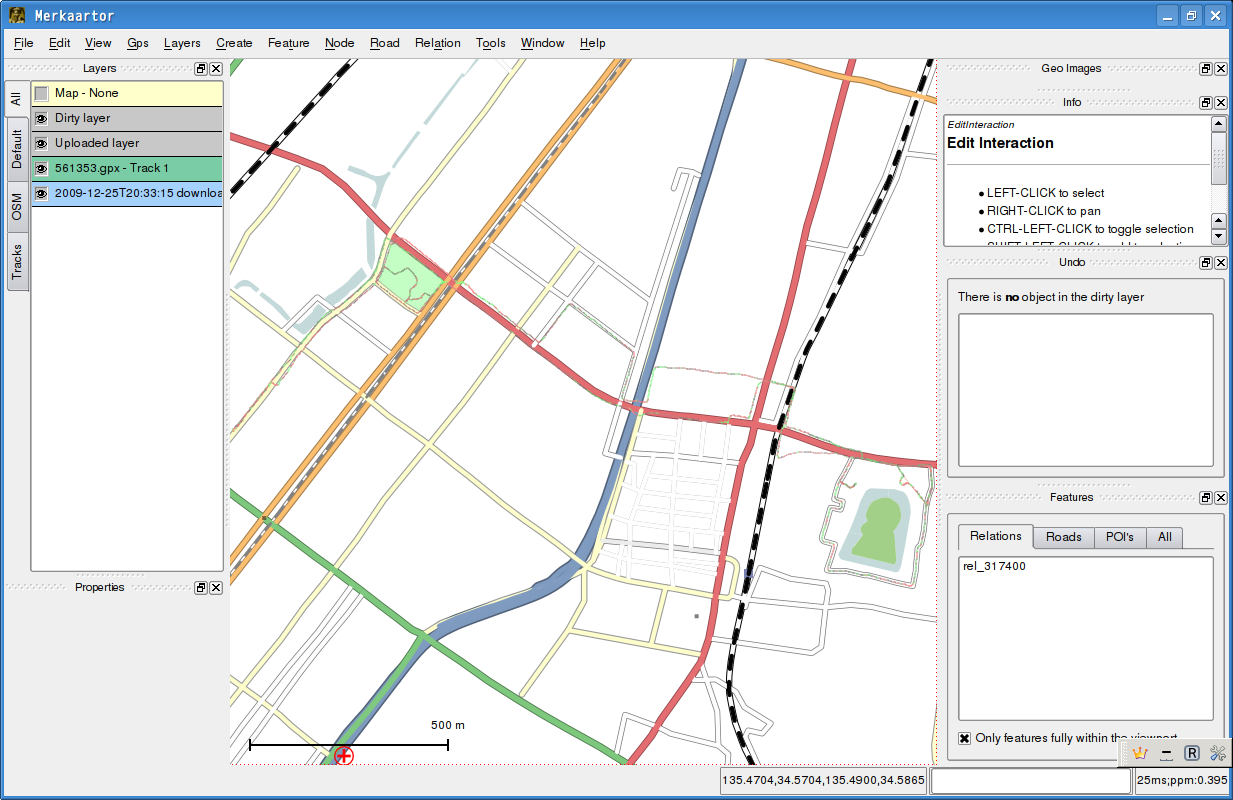
\includegraphics[scale=0.28]{image200912/debianosm7.png}
\end{wrapfigure}

 Merkaartor は、OSM の作図ソフトです。
 OSM 向けの作図ソフトは、大きく3つあります。

\begin{enumerate}
 \item Potlatch \\
Potlatch は、フラッシュベースの作図ソフトで、Web ブラウザがあれば使う事が
出来ます。
 \item JOSM \\
JOSM は、Java で書かれた作図ソフトで多機能です。Java 版なので、Debian で
も Windows でも動きます。
 \item Merkaartor
Merkaartor は、Qt ライブラリを使って書かれた作図ソフトです。
JOSM と同じく Debian でも Windows でも動きます。
\end{enumerate}

どれがお奨めか、これは3つとも自由に使えるソフトですので、3つ試して一番
自分に合うものを選んで下さい。一概にどれが良い・悪いと言うのはありません。
ただ、私見ですが、Merkaartor は多機能で無い分、初心者にとってはかえって分
かりやすいと考えています。

Debian lenny に入っている Merkaartor は少しバージョンが古く、Debian
Backportsサイト(\url{http://www.backports.org/}) から、出来るだけ新しい
Merkaartor をインストールすると良いでしょう。

\subsubsection{navit}

「deb \url{http://navit.latouche.info/debian} lenny main」を、/etc/apt/sources.listに追加します。

\begin{commandline}
# gpg --recv-keys CB229096
# gpg --export -a CB229096 | apt-key add -
# apt-get update
# apt-get install navit
\end{commandline}

\begin{wrapfigure}{r}{23zw}
 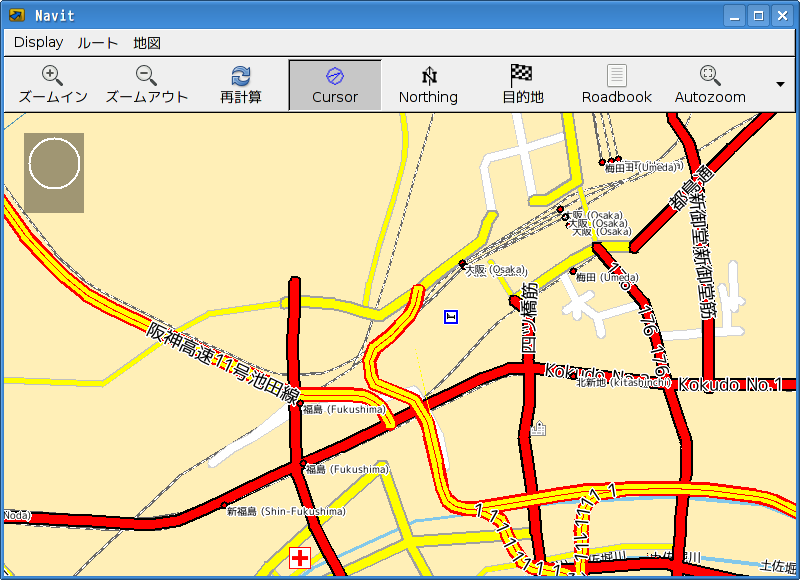
\includegraphics[scale=0.38]{image200912/debianosm8.png}
\end{wrapfigure}

navit は、OSM 地図データに対応した地図表示ソフトです。gpsd が必要で、
gpsd から現在の緯度経度を取得し、OSM 地図データと重ね合わせ表示する事が出
来ます。
navit は OSM 地図データを事前に取り込む方法ですので、ネットが使えないオフ
ライン環境下でも地図を見る事が出来ます。

筆者は Debian Lenny をインストールした EeePC に、gpsd と navit をインストー
ルし、大阪から新潟まで使ってみたことがあります。
実際の走行は、殆どが高速道路ですので、ナビと言うほどのものはありませんで
したが、私が念願としていた、「自由な OS で、自由なソフトで、自由な地図デー
タでナビをする」と言う事が達成できた瞬間でした。

筆者はまだまだ、Debian System は初心者の域を出ません。もし Debian System
にあるパッケージで、良いものがありましたら紹介下さい。

\subsection{筆者の GPS ログ機器}

筆者は、主に2台の GPS 受信機を使ってログを取っています。

\subsubsection{GT-31}

GT-31 は、小型防水の GPS ロガーで、バイクに取り付けることが出来ます。

GT-31 の良い所は、GPS ログを SD カードに保存する事が出来るので、記録容量
が SD カードの容量次第で大きく出来る点です。また、IPX7相当の防水性能があ
ります。IPX7 相当の防水機能とは、1m の水中に、30分間沈んでいても内部に水
が入らない構造を指します。

筆者は GT-31 の SDカードに、NMEA-0183 の形式で保存しています。

\subsubsection{HI-406BT}

GT-31 と併用して、HI-406BT も使っています。

HI-406BT は、純粋な GPS 受信機であり、この機器自身にログ機能はありません。
HI-406BT は Bluetooth インターフェースなので、筆者は Bluetooth 付きの
PDA や PC に、これも NMEA-0183 の形式で保存するようにしています。

\subsubsection{HOLUX m-241}
HOLUX m-241 は、単3乾電池一つで動作する小型 GPS ロガーです。

小型でありながら、ロガーとしての記録容量が大きく、130,000点のログが可能で
す。加えて Bluetooth に対応しています。筆者が OSM に作図し始めた頃は、こ
の m-241 でログを取っていました。
残念な事に、筆者の m-241 は壊れてしまい、今は GT-31 と HI-406BT を併用し
ています。

GPS は、余裕があれば2台欲しいです。白地図を作図するときは、やはりGPSログ
から作図しますので、ログ取り忘れはかなり寂しい事になります。

GT-31 は、GPS ログしない。と言う選択肢が無く、常にログします。m-241 は、
ボタンのトグルでログする・しないを選択できますが、ついうっかり忘れてしま
う事がありますので、GPS ログを取る・取らないが選択できる GPS 受信機を使う
場合、GPS ログ状態がすぐに確認できるものを選ぶと良いでしょう。

\subsection{GPSロガー選び方ノウハウ}

\subsubsection{DOP (Dilution of Precision - 精度低下率) が分かるものを選ぼう}

GPS レシーバは、「GPS 衛星から現在位置をもらう」のではなく、GPS 衛星から
正確な時刻と GPS 衛星の移動情報を元に、「GPS レシーバが自力で現在地を計算
する」仕組みです。

そのため、計算結果から、精度がどれくらい低下しているかを判断する事が出来ます。
これは GPS 衛星一つから現在地を知るのではなく、最低3つの GPS 衛星から現
在地を計算するためです。

DOP は、小さければ小さいほど精度が良い事を示します。この DOP は、受信した
(計算に選択した)GPS 衛星のばらけ具合によります。DOP には、水平方向の
HDOP、垂直方向の VDOP 、位置を示す PDOP があります。

下記のページに記載がありますが、OSM は、PDOP の値は 4 より下、2 より下な
らかなり良く固定されているとあります。

\url{http://wiki.openstreetmap.org/wiki/Ja:Recording_GPS_tracks}

筆者自身、作図のために GPS ログを取る時は、DOP 値には相当気を使っています。

GPS ロガー "GT-31" は、DOP 値を表示することが出来ますので、筆者が GPS ロ
グを取る時は、現在の緯度経度よりも、DOP 値を表示させるようにしています。
DOP をログする GPS ロガーを使用した場合、GPX ログにも DOP を残す事が出来
ますので、JOSM や Merkaartor でも視覚的に確認できます。

NMEA-0183 センテンスの場合、GSA センテンスがこれにあたります。

\subsubsection{外部アンテナが付けられるのと付けられないのでは大違い}

GPS 受信機には、外部アンテナを取り付ける事が出来るものがあります。
筆者は "HI-406BT" と言う Bluetooth GPS レシーバも使うのですが、これには外
部アンテナを取り付けることが出来ます。

外部アンテナを取り付けることで、GPS 信号の感度が上がり、精度が向上します。
また、外部アンテナは概ね防水型ですので、外部アンテナを車の屋根に取り付け、
天候に左右されずにログを取る事が出来ます。

\subsubsection{測位精度の誤差}

最近の GPS 受信機は精度が向上し、概ね「10m 2drms」の範囲です。
「2drms」と言うのは、これを半径とする円内に、およそ 95\% の測位点が入る事
を表します。
10m 2drms ならば、半径10m の円内に 95\% の測位点が入る事を示します。

半径10m だと、地図として使うのに誤差としては大きいかも知れませんが、DGPS
だと 5m 2drms にまで誤差が少なくなるものもあります。
GPS 受信機を購入する時は、この 2drms の値は確認しておくと良いでしょう。

\subsubsection{バッテリーの持ちと形状}

1時間程度のログであればあまり問題はありませんが、バイクツーリング等でほ
ぼ1日乗りっぱなしで GPS ログを取る場合、GPS 受信機のバッテリーも気になり
ます。

GPS 受信機のバッテリーの持ちもそうですが、バッテリーの形式、例えば乾電池
か専用電池かも、利用形態に応じて考える必要があります。

最近の個人用 GPS 受信機は、USB で充電できるものがあります。これと携帯の充
電器にあるような、乾電池の電力を USB に変換して出す充電器を併用する事で、
専用電池でもバッテリーを気にせずに使う事が出来ます。

せっかくの GPS 受信機も、バッテリーが干上がると、mapper にしてみるととて
も寂しい事になりますので、バッテリーの持ちや、形状は確認しておくと良いで
しょう。

\subsection{おわりに}
OpenStreetMapは、日本ではまだまだ認知の低いプロジェクトですが、Debian
System とも十分親和性の高いプロジェクトですので、興味を持って頂けたならう
れしいです。



\dancersection{関西 Debian 勉強会\newline2009年度各種イベント開催実績と総括}{倉敷・佐々木・野方}
\index{2009ねん@2009年}
\index{かんさいでびあん@関西Debian勉強会}

\subsection{運営状況}

関西は運営に関わっている人に学生が多いので、いろいろ無理をお願いする場
面も多かったような気がします。

\subsubsection{勉強会全体}

今年度途中(7月)より、運営担当が山下尊也から倉敷・佐々木・野方の三名体制
に交代しました。これは山下の身辺が多忙になり身動きがとれないという理由
からです。幸い、以前より分担に向け運営の見直しを進めていたこともあり、
大きな混乱もなく継続することができました。

年度当初、ライブ中継に若干盛り上がりを見せましたが、その後、うまく継続
できませんでした。問題としてはIPアンリーチャブルな会場をメインにしてい
ることと、中継の実作業を担っていた人が運営側にシフトし、余力を回せなく
なっていることが原因と思われます。

5月には神戸市を中心とした関西地域の新型インフルエンザ流行により、勉強
会を中止する出来事がありました。
社会的な要因により勉強会開催の判断を迫られる状況は初めてでしたが、こう
いう事は二度とあって欲しくないですね。

9月は京都リサーチパークにお邪魔して勉強会初の京都で開催しました。会場を
変えると、いつもとは違う参加者も増えるので、たまに場所を変えるのもよい
のではと思いました。

講師については現状、固定化している中、継続して常連参加者への講師依頼を
するほかに、DMCを取り入れたり、LT発表も可能な参加者自己紹介の常設な
どをおこないました。

LT発表可能な参加者自己紹介は、話題にバリエーションが加わったなど興味深
いこともあった反面、年度後半は関西の勉強会参加者も参加している Open
Street Mapにトピックを持っていかれてしまった感もあり、うまくバランスを
取る必要がありそうです。

また、今年度は佐々木、山下の 2 名が Package Maintainer として
Debian の New queue に新しくパッケージを送り込みました。来年も
この流れを維持できればと思います。

\subsubsection{扱ったテーマ}

勉強会の内容としては、パッケージ開発自体に加えて、Debian の体制にまつわ
る話(gpg や mentors など)や、周辺ツールの利用(bash や reportbug や gdb
など)をとりあげました。
来年度のテーマについては、年末年始に相談をする予定をしています。

翻訳関連では、東京での流れに乗りDDTSSのハンズオン実習をしましたが、予想
外に反応がありました。もともと需要があったのか、実習したことで身近になっ
たのか、はよくわかりませんが…。

\subsubsection{イベント関連}
例年通り、夏のオープンソースカンファレンスKansai@Kyoto(OSC)と、秋の関
西オープンフォーラム(KOF)に出展しました。

セッションでは、OSCでは大浦さんによるDebian GNU/kFreeBSDについて、KOFで
は矢吹さんにDDになるまでの軌跡をお話してもらいました。
矢吹さんは、関西Debian勉強会立ち上げの立役者なので、できれば勉強会にも
来て欲しいところですが、最近は、なかなかご多忙で難しいとのことです。

また、四国ではじまったオープンフォース勉強会 \footnote{
\url{http://openforce.project2108.com/}}と、岡山でのオープンセミナー
@岡山 \footnote{\url{http://openseminar.okaya.ma/}} に、野方が参加して
Debian Liveやノウハウの紹介などを行いました。

\subsection{開催実績}

関西Debian勉強会の出席状況を確認してみましょう。
グラフで見ると\fgref{fig:kansaipeoplechart}になります。
表で見ると\tbref{tab:count2009kansai} です。

\begin{figure}[h]
 \begin{center}
  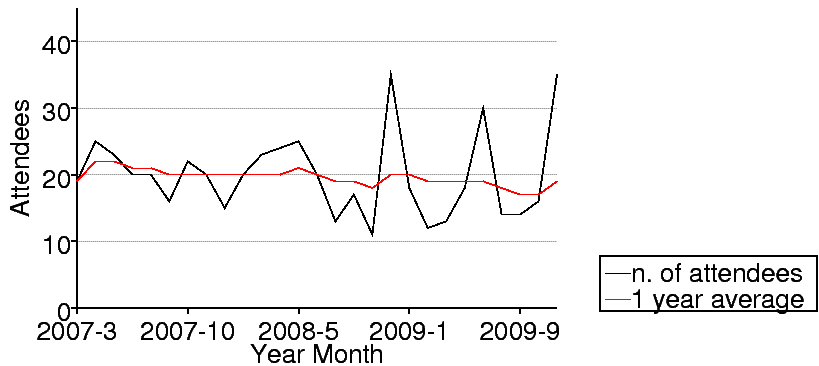
\includegraphics[width=1\hsize]{image200912/kansai.png}
 \end{center}
\caption{関西の参加人数推移}
\label{fig:kansaipeoplechart}
\end{figure}

\begin{table}
\begin{minipage}{0.5\hsize}
 \caption{関西Debian勉強会参加人数(2007年)}\label{tab:count2007kansai}
 \begin{center}
  \begin{tabular}{|l|c|p{10em}|}
 \hline
 & 参加人数 & 内容 \\
 \hline
2007年3月 & 19 & 開催にあたり \\
2007年4月 & 25 & goodbye、youtube、プロジェクトトラッカー\\
2007年6月 & 23 & 社会契約、テーマ、debian/rules、bugreport\\
2007年7月 & 20前後 & OSC-Kansai \\
2007年8月 & 20 & Inkscape、patch、dpatch\\
2007年9月 & 16 & ライブラリ、翻訳、debtorrent\\
2007年10月 & 22& 日本語入力、SPAMフィルタ\\
2007年11月 & 20前後 & KOF \\   
2007年12月 & 15& 忘年会、iPod touch\\   
 \hline
  \end{tabular}
 \end{center}
\end{minipage}
\begin{minipage}{0.5\hsize}
 \caption{関西Debian勉強会参加人数(2008年)}\label{tab:count2008kansai}
 \begin{center}
  \begin{tabular}{|l|c|p{10em}|}
 \hline
 & 参加人数 & 内容 \\
 \hline
2008年2月 & 20 & PC Cluster, GIS, \TeX \\
2008年3月 & 23 & bug report, developer corner, GPG \\
2008年4月 & 24 & coLinux, Debian GNU/kFreeBSD, sid \\
2008年5月 & 25  & ipv6, emacs, ustream.tv\\
2008年6月 & 20  & pbuilder, hotplug, ssl\\
2008年8月 & 13  & coLinux \\
2008年9月 & 17  & debian mentors, ubiquity, DFSG\\
2008年10月 & 11  & cdbs,cdn.debian.or.jp \\
2008年11月 & 35  & KOF \\
2008年12月 & ?  & TeX資料作成ハンズオン\\
 \hline
  \end{tabular}
 \end{center}
\end{minipage}
\begin{minipage}{0.5\hsize}
 \caption{関西Debian勉強会参加人数(2009年)}\label{tab:count2009kansai}
 \begin{center}
  \begin{tabular}{|l|c|p{10em}|}
 \hline
 & 参加人数 & 内容 \\
 \hline
2009年1月 & 18 & DMCK, LT \\
2009年3月 & 12 & Git \\
2009年4月 & 13 & Installing sid, Mancoosi, keysign \\
2009年6月 & 18 & Debian Live, bash\\
2009年7月 & 30? & OSC2009Kansai \\
2009年8月 & 14 & DDTSS, lintian \\
2009年9月 & 14 & reportbug, debian mentors\\
2009年10月 & 16 & gdb, packaging \\
2009年11月 & 35 & KOF2009 \\
2009年12月 & ?? & GPS program, OpenStreetMap \\
 \hline
  \end{tabular}
 \end{center}
\end{minipage}
\end{table}

\clearpage

\dancersection{今後の予定}{Debian JP}

\subsection{次回の関西Debian勉強会}
次回は、2010年1月の関西Debian勉強会は2010年1月24日に大阪港区民センターで
おこないいます。いつもの福島区民センターではないのでご注意ください。

\subsection{オープンソースカンファレンス Kansai @ Kobe 2010}
2010年3月13日土曜日にJR神戸駅すぐそばの神戸市産業振興センターにて、オー
プンソースカンファレンス Kansai @ Kobe 2010が開催されます。
関西Debian勉強会では、現在参加を検討しています。

% 冊子にするために、4の倍数にする必要がある。
% そのための調整
\dancersection{メモ}{}
\mbox{}\newpage
\mbox{}\newpage
\mbox{}\newpage

\printindex
 \cleartooddpage

 \begin{minipage}[b]{0.2\hsize}
  \rotatebox{90}{\fontsize{80}{80} {\gt 関西デビアン勉強会} }
 \end{minipage}
 \begin{minipage}[b]{0.8\hsize}

 \vspace*{15cm}
 \rule{\hsize}{1mm}
 \vspace{2mm}
 
\includegraphics[width=2cm]{image200502/openlogo-nd.eps}
 \noindent \Large \bf Debian 勉強会資料\\ \\
 \noindent \normalfont \debmtgyear{}年\debmtgmonth{}月\debmtgdate{}日 \hspace{5mm}  初版第1刷発行\\
 \noindent \normalfont 関西 Debian 勉強会 (編集・印刷・発行)\\
 \rule{\hsize}{1mm}
 \end{minipage}

\end{document}
